\documentclass[12pt,letterpaper]{article}
\usepackage{graphicx}
\usepackage{geometry}
\usepackage{setspace}
\usepackage{anyfontsize}
\usepackage{parskip}
\usepackage{indentfirst}
\usepackage{amsmath}
\usepackage{cite}
\usepackage{listings}
\usepackage{color}
\usepackage{textcomp}
\usepackage{float}
\usepackage[utf8]{inputenc}
\usepackage{natbib}


\geometry{letterpaper, portrait, margin=1in}
\doublespace
\title{The Representation, Generation and Industry Application of B\'ezier Curves}
\author{Tynan Purdy}
\date{\vspace{-5ex}}

\graphicspath{{../Diagrams/}}

\definecolor{codegreen}{rgb}{0,0.6,0}
\definecolor{codegray}{rgb}{0.5,0.5,0.5}
\definecolor{codepurple}{rgb}{0.58,0,0.82}
\definecolor{backcolor}{rgb}{0.95,0.95,0.92}

\lstdefinestyle{scheme}{
    backgroundcolor=\color{backcolor},
    commentstyle=\color{codegreen},
    keywordstyle=\color{blue},
    numberstyle=\tiny\color{codegray},
    stringstyle=\color{codepurple},
    basicstyle=\footnotesize\ttfamily,
    breakatwhitespace=false,
    breaklines=true,
    captionpos=t,
    keepspaces=true,
    numbers=left,
    numbersep=5pt,
    showspaces=false,
    showstringspaces=false,
    showtabs=false,
    tabsize=2
}

\lstset{style=scheme}


\begin{document}
\large
\parindent=0.5in
{\fontsize{12}{14.4}
	{\singlespace
	\pagenumbering{gobble}
	\maketitle
	\begin{center}
	\vspace{4mm}
	002129-0004 \\
	\vspace{4mm}
	Extended Essay \\
	\vspace{4mm}
	Mathematics \\
	\vspace{4mm}
	May 2019 \\
	\vspace{4mm}
	Words: \\
	\end{center}
	}
}	

\newpage
\pagenumbering{arabic}
\begin{abstract}
hi Curves are everywhere. In architecture, in objects, in books. Consider how many of those curves existed at some point on a computer. Graphic designs, 3D models of products, paper documents, so much of our carpentered world is rendered on a computer before it ever sees the third dimension. Computer-Aided Design programs have taken over the manufacturing industry with versatile and extensive software packages that simulate any physical object right on the computer. Graphic design programs are at the source of every print and screen display. But these computer programs must be able to produce curved lines and surfaces in a computationally efficient way, or else producing all the curves used every day would bring computer hardware to its knees. A French automotive engineer by the name of Pierre B\'ezier implemented an efficient and easily adjustable method of digital curve rendering called the B\'ezier curve. His method of curve drawing has made its way into countless digital mediums, including 3D and 2D design software, digital typefaces, and more.
\end{abstract}

\newpage
\tableofcontents

\newpage
\section{Introduction}
The Information Age has introduced some drastic changes to the way humans communicate and exchange information. Over the past several hundred years, the dissemination of information has benefited from inventions such as Gutenberg’s printing press and the digital computer have revolutionized the way we encode and decode information. Advances in communication lie at the heart of the development of civilization. Before the printing press made books and published works accessible to the world, books were available only to monks and scholars, who made up a very small part of the population. Books and papers were handwritten by scribes, a tedious process subject to human error. With most information behind closed doors, education, even literacy, was an uncommon skill. 

Information technology (IT) has real effects. European cities that made use of the printing press in the 16th century grew 60\% faster than comparable cities that did not. \citep{press} Books, libraries, newspapers, all became publicly acquirable resources. When information is more accessible, more ideas can be shared and innovated on. Medical and hygienic practices and advancements can be mass produced for everyone to implement lifesaving habits. Informed populations carry more democratic power to have their own opinions based on personal research as opposed to listening to some omnipotent higher authority. Abundance of information and sharing of information leads directly to a wide myriad of benevolent consequences lending to a healthier society. 

IT can take many forms, some rather unexpected, and each with their own tradeoffs. Scrolls, paper books, ink pens are all forms of IT. Scrolls were the most efficient method of storing information for centuries. Paper books, an improvement on the scroll, are able to hold many more pages per unit of volume than scrolls but can be difficult to manufacture without the right tools. The pen has gone through many innovations. The original feather and ink were a functional way to write, despite requiring frequent dips in the ink. The feather’s ability to hold ink was less than desirable, only able to write for a word or two between ink dips. Fountain pens held ink for far longer, allowing the user to be much more efficient with their writing. Innovations in IT allow for more storage and bandwidth for transferring information, as well as making content creation accessible to the public. Handwritten letters are an invaluable source for historians. 

Modern information technology has grown to an enormously complicated and diverse field due to recent globally revolutionizing inventions: the digital computer and the internet. In the 21st century, IT encompasses computer networking, servers, online communication mediums like Twitter and Gmail, photos, videos, I/O ports, smartphones, and even file formats. Some areas of IT are so new and unique that world governments are still figuring out how to regulate it. Net Neutrality protections give internet users the right to communicate with whoever they chose on the internet without interference from Internet Service Providers. Net Neutrality hasn’t been particularly successful in recent years, but there are good regulations that are already in effect. In April of 2018, the European Union passed the General Data Protection Regulation (GDPR), which strictly defines what internet companies can do with user data and gives users specific rights to their data. Because the internet is so global, unlike communication mediums of the past, regulations like GDPR are treated as if they are worldwide rules, even though they are only enforced in Europe. Companies would rather have one universal policy for their users than have to deal with different policies for users in different countries. IT is a deep and difficult topic, with many branches of influence. However, there is a particular IT innovation that is used across the entire internet, and almost every form of communication today, the Bézier curve. 

Bézier curves, a mathematical process for drawing curves, has found its way into the lifeblood of modern communication, digital graphics and text. Every screen in the world is almost constantly using Bézier curves to draw whatever it is displaying. Most technology users don’t know what Bézier curves are, despite looking at them every day for hours on end.  The lines of text on this very page were drawn using Bézier curves. The art on billboards were rendered with Bézier curves as they were printed. The ability to render text characters virtually instantly has contributed to the content boom of the internet. The following pages will describe what Bézier curves are, where they came from, and exactly how they are used to deliver words and shapes to the digital world.


\section{B\'ezier Curves}

\subsection{Where did B\'ezier Curves come from?}
While the mathematics behind Bézier curves has existed for decades before computers were invented, it was the French automotive engineer, Pierre Bézier (1910-1999), who popularized the method for digital curve and surface drawing. B\'ezier was a mathematician and head of design at Renault, a Paris based automaker. (Farin, Hoschek and Kim) Before the origin of these special curves is revealed, it must be understood why curves are important and so difficult to procure digitally.

Curves have been used in mechanical design for hundreds of years, and for good reason. They give a smooth, attractive form that is not only more inviting to the touch, but also lends itself toward aerodynamics. Curves are perfect for effortlessly passing through fluids such as air and water.

\begin{figure}[H]
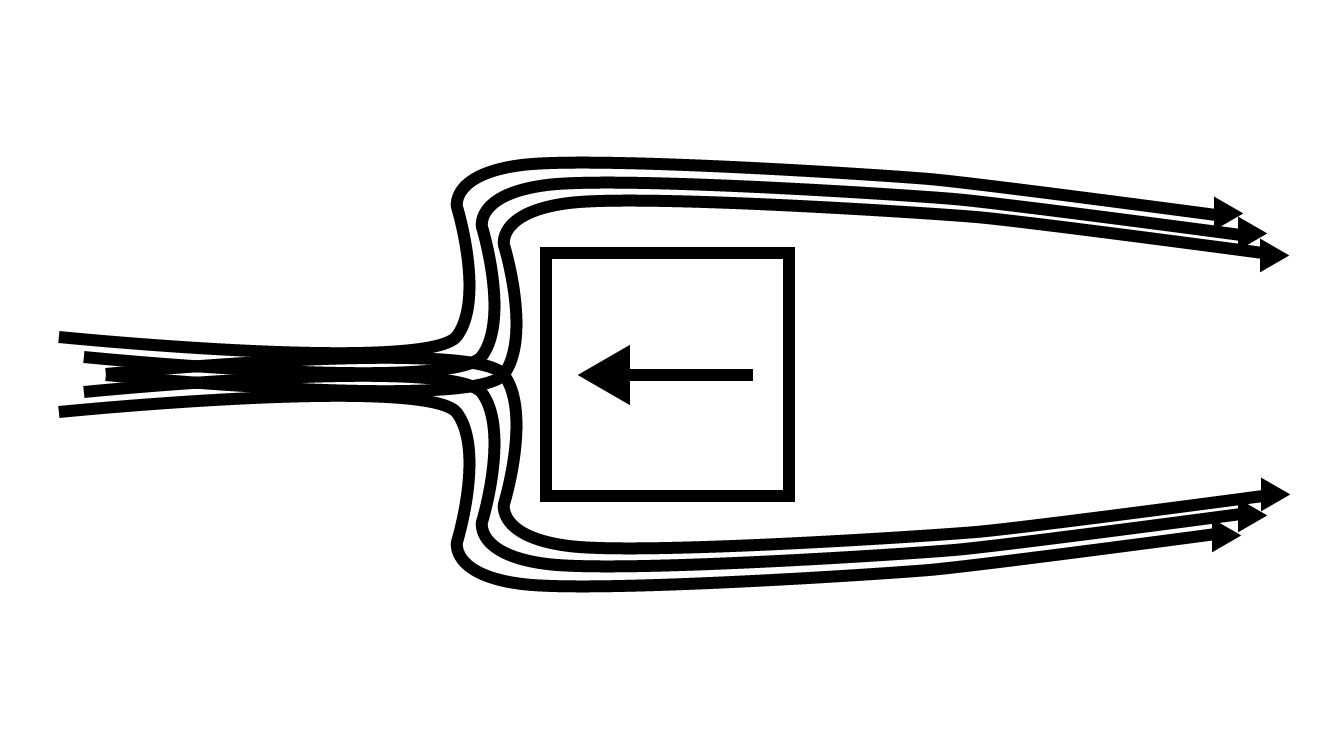
\includegraphics[width=12cm]{aero-square}
\centering
\caption{Fluid passing around a cornered object. Fluid must be redirected harshly to get around the square object, creating excess friction and heat.}
\end{figure}

\begin{figure}[H]
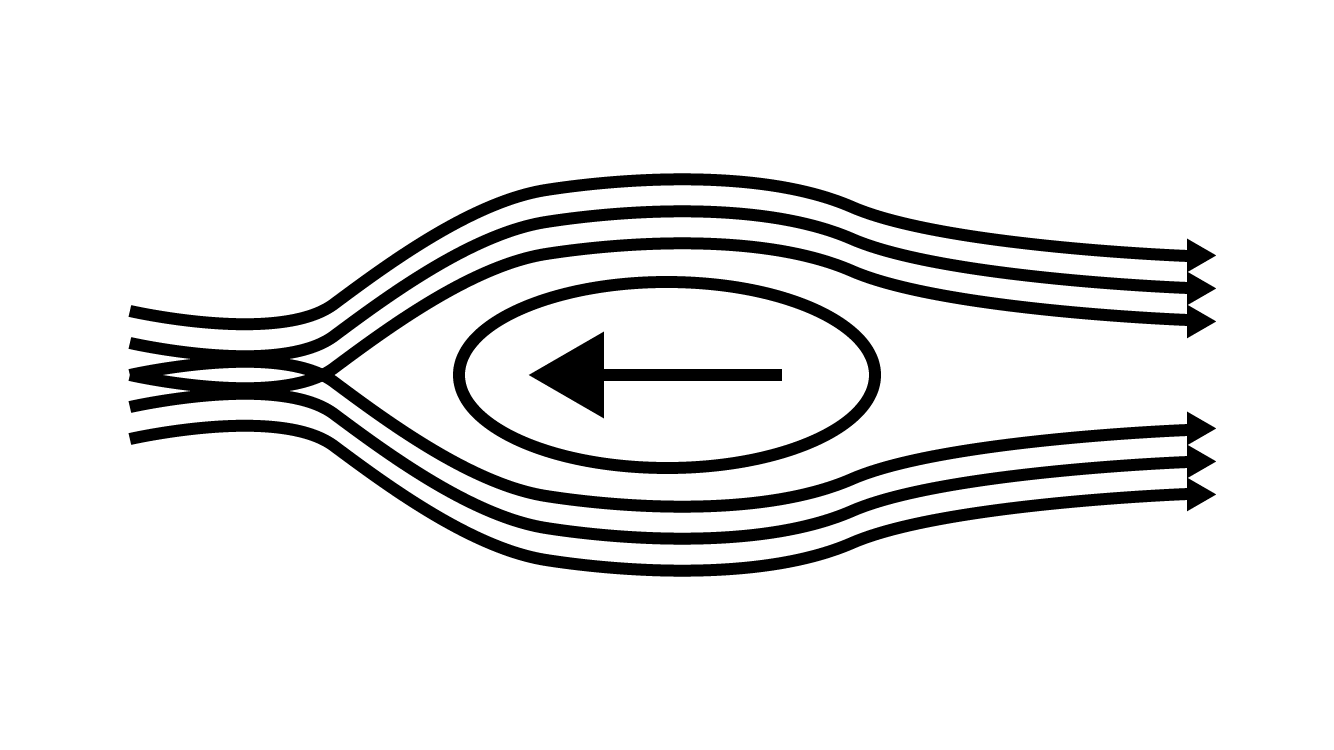
\includegraphics[width=12cm]{aero-curve}
\centering
\caption{Fluid passing over a curved object. The fluid is redirected less to pass around the object, resulting in less friction and heat than the square object.}
\end{figure}

Unsurprisingly, aerodynamics in air and water accounts for the primary uses of curved surfaces both in ancient Rome and today: boats, planes, and cars. Consider the cars seen on the road today. Even an astute observer would have a hard time finding a perfectly flat surface or hard corner anywhere on the vehicle. Geometric patterns are so popular in the 2010s, yet they haven’t made their way to cars, simply because curves are so energy efficient compared to straight lines and corners that there is no compelling reason to abandon them. 

Curves are also much safer than square edges and corners. Even objects that appear to have square corners often have a small filet to smooth them out and avoid potential accidental cuts or scratches. Curves’ safety properties arise from the same traits as its aerodynamic properties. An angled edge is more able to split open a solid that a curved edge, the reason knives must be sharp to function properly. The concern of safety against hard edges is addressed extensively in the manufacturing space. A wide variety of tools exist purely to reduce sharp edges to a smooth and save curve. Most subtractive machining tools leave a straight edge after a linear cut, as well as small bits of debris still attached to the edge called burrs. Belt sanders, files, deburring tools, countersink bits, and sanding blocks are all different tools used to round or smooth edges after a cut and remove burrs.

When considering a user of an object or product, curves are an easy way to make the user feel at ease and comfortable with the product, as well as keep them safe. 

Curved edges and surfaces clearly have their benefits. As shown above, there are ways to add curves to a cornered object, but it would be better to include curves in the original design. With manually operated tools, creating a curve is not particularly difficult. The human brain can describe and instruct the hands to use tools to make any shape or surface imaginable that the tool is capable of creating. Handcrafted wood objects can be curved with a chisel and some sanding. In the car manufacturing industry, most auto bodies are modeled at full scale in clay during the design phase. Handcrafting is fine for many purposes, but when the end goal of a design is to mass produce it, at some point the shape of the object must be described by a computer. Manually operated tools are time consuming and labor intensive to make thousands of identical parts for mass production, which is not feasible for large scale manufacturing. Computer numerical control (CNC) tools have solved the mass production issue by allowing tools to be programmed to execute precise cuts perfectly and repeatably. CNC tools require far less attention from a human operator and produce consistent machining, perfect for mass production. The catch is, since the machine is computer controlled, the computer must be able to describe the cuts it is supposed to make, which means they must be described mathematically. Pierre B\'ezier was one of the first engineers to address the need for digital rendering of physical parts, and so began development of the B\'ezier curve for Renault. B\'ezier was not the first, nor the only engineer to work on a mathematical curve algorithm for computers, but his was the widely adopted method. The famous de Casteljau’s algorithm was developed for Citroën, a competing auto company in Paris. His algorithm was kept secret for years after its development in the ‘60s. (Farin, Hoschek and Kim)


\subsection{What are B\'ezier Curves?}
Put simply, a B\'ezier curve is a curve defined by a set of control points. These control points are not necessarily intersected by the curve but they determine its shape.
\begin{figure}[H]
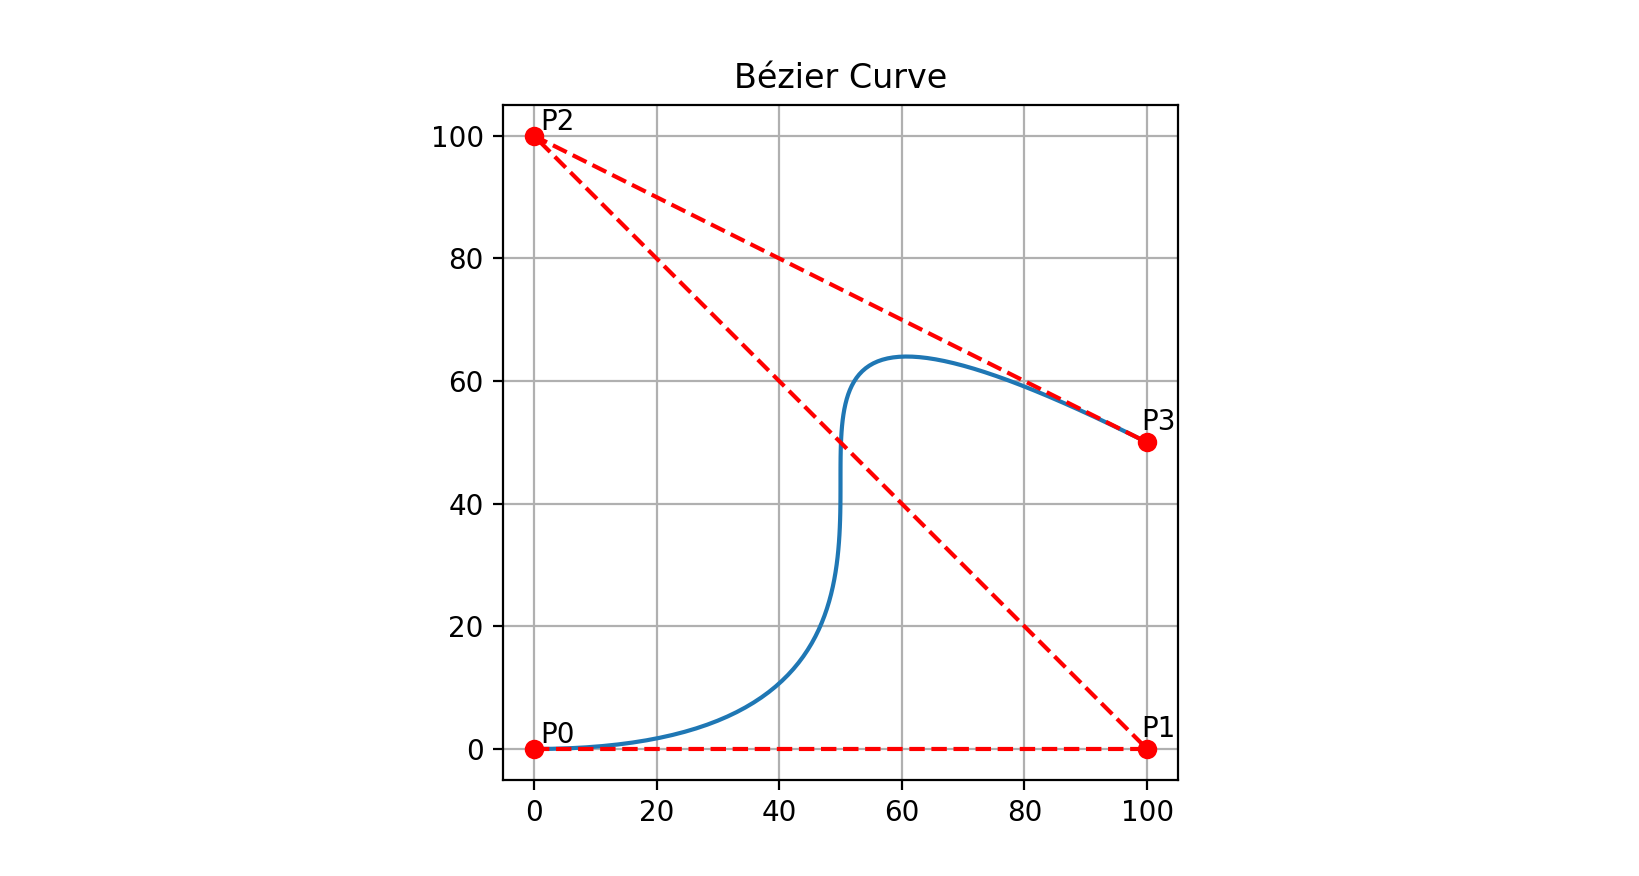
\includegraphics[width=15cm]{Figure_1}
\centering
\caption{B\'ezier curve with 4 control points.}
\end{figure}
Consider Figure 4, a curve with four control points: $P_0, P_1, P_2,$ and $P_3$. $P_0$ and $P_3$ are the endpoints of the curve, so they will be intersected by the curve. $P_1$ and $P_2$ will not be intersected by the curve. They do ‘pull’ the curve in their direction. Placing $P_1$ closer to a line between $P_0$ and $P_3$ will reduce the bend towards $P_1$.
\begin{figure}[H]
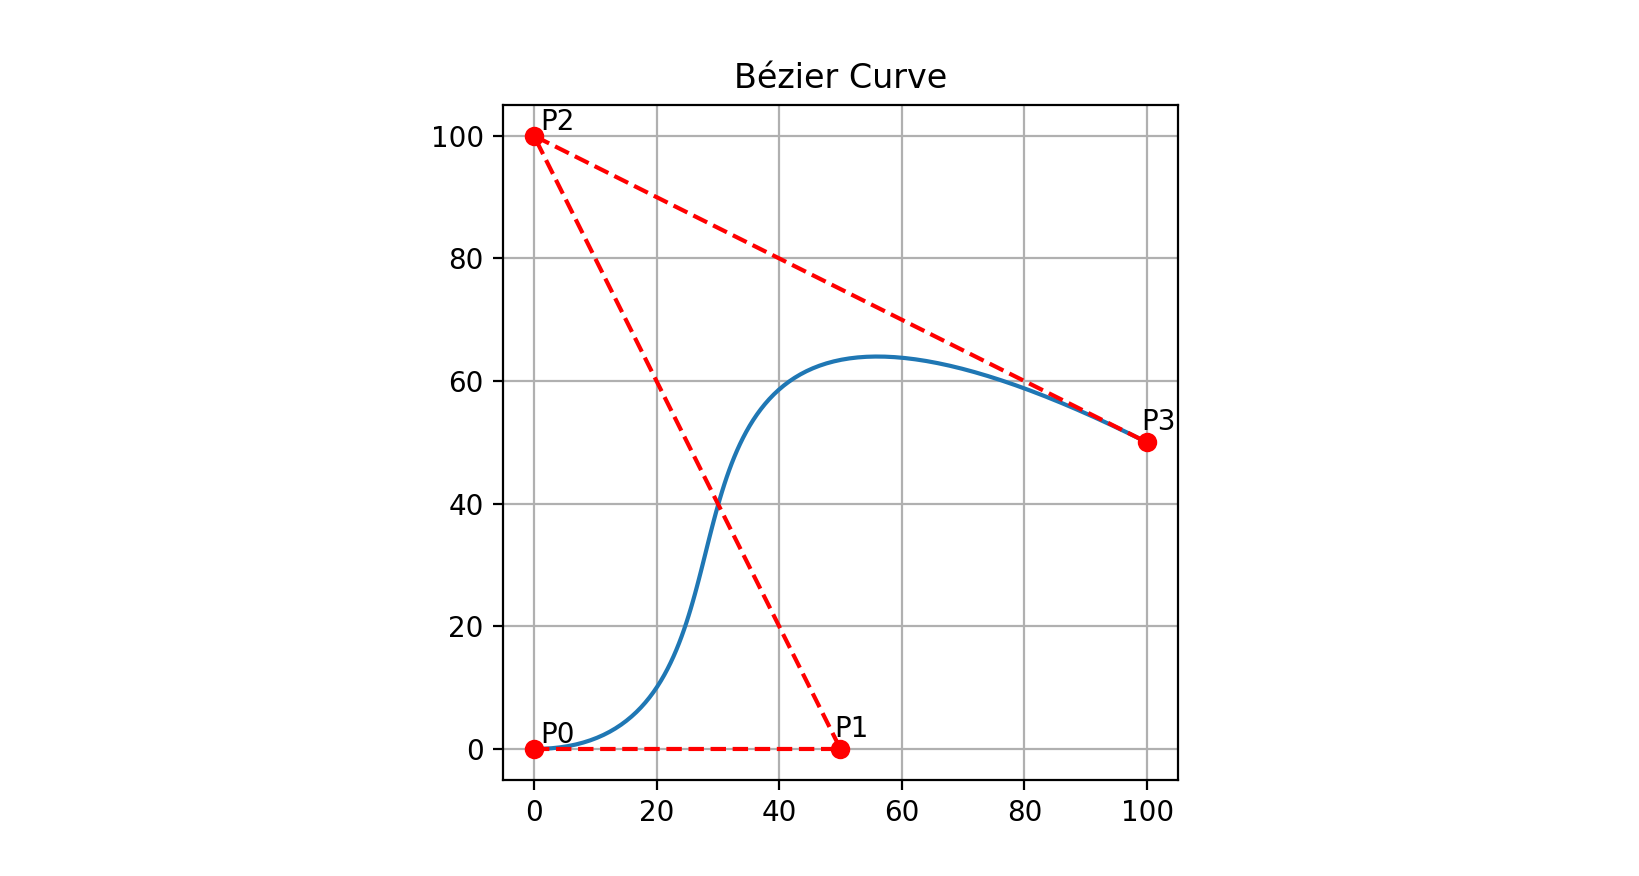
\includegraphics[width=15cm]{Figure_2}
\centering
\caption{Demonstration of how control points influence the curve. The closer the control points are to forming a line, the less curvature.}
\end{figure}
The behavior of the curve in relation to its control points comes from the properties of the equation that defines the curve. B\'ezier curves are defined by a parametric equation of Bernstein polynomials. A parametric equation uses a parameter as a determining factor of the result of the function. While traditional graphed functions use an x coordinate to solve for a y coordinate, the parameter is used to define x and y individually. 
Take Equation 1 below. The parametric equation uses the parameter t and two control points, $P_0$ and $P_1$. The equation is solved given t from 0 to 1. At $t=0$, the result is equal to $P_0$, and at $t=1$ it is equal to $P_1$.
$$B(t) = P_0 + t(P_1 - P_0)$$
In order to graph Equation 1 as a linear B\'ezier curve (don’t mind the paradox, it works the same way), two control points must be designated, for instance $P_0$(1, 1) and $P_1$(2, 3). Then, the coordinates will be substituted into the parametric equation for x and y.
$$x(t) = 1 + t(2-1)$$
$$y(t) = 1 + t(3-1)$$
Evaluating $x(t)$ and $y(t)$ from 0 to 1 produces coordinate points on the ‘curve’ shown below. 
\begin{figure}[H]
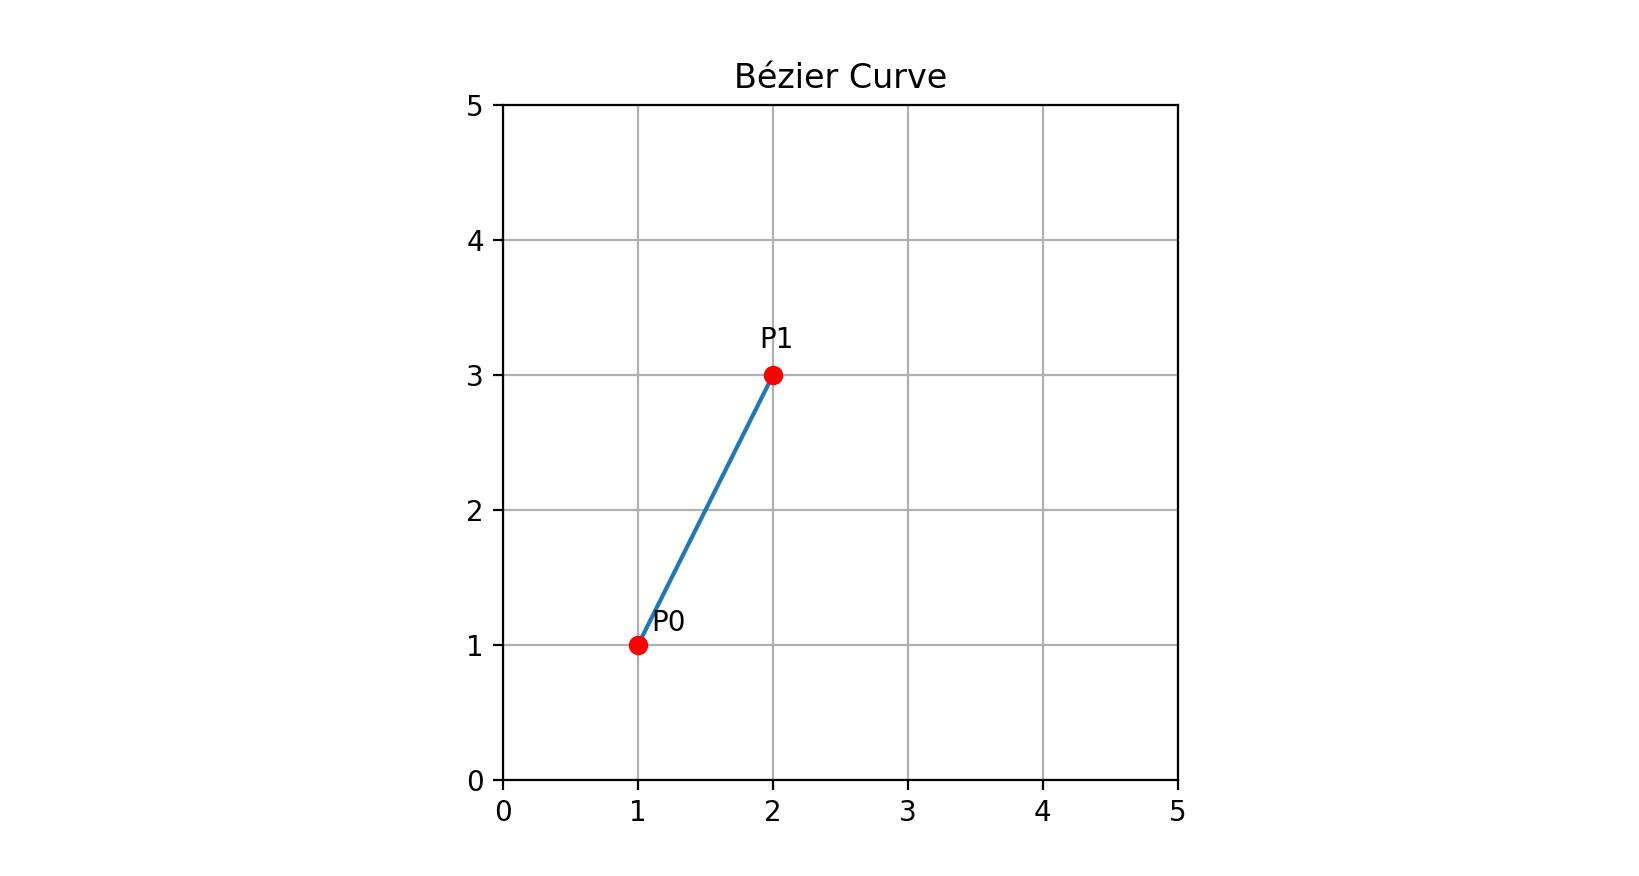
\includegraphics[width=15cm]{Figure_3}
\centering
\caption{Linear B\'ezier curve.}
\end{figure}
As t increases from 0 to 1, the coordinates produced become further from $P_0$ and closer to $P_1$ because $P_0$ is getting subtracted away and $P_1$ is being added at equal rates. 

Drawing a simple line with a parametric equation isn’t particularly impressive. However, when the equation is rearranged to be a Bernstein polynomial, the formula can easily be adapted to accommodate more dimensions. Equation 1 is a 1st order Bernstein polynomial with the control points as coefficients if rearranged like below.
$$B(t) = (1-t)P_0 + t P_1$$
Each term in the Bernstein polynomial is matched sequentially with a control point as a coefficient to create formulas for higher order polynomials (See Table 1).

\begin{table}[H]
\centering
\begin{tabular}{ | c | c c | c | }
\hline
$B_{n,m} (t)$ & Bernstein Term & CP Coefficient & Complete Term \\
\hline
$B_{1,0}$ & $1-t$ 		& $P_0$ & $(1-t)P_0$ 	\\
\hline
$B_{1,1}$ & $t$ 		& $P_1$ & $tP_1$ 		\\
\hline
$B_{2,0}$ & $(1-t)^2$ 	& $P_0$ & $(1-t)^2P_0$ 	\\
\hline
$B_{2,1}$ & $2(1-t)t$ 	& $P_1$ & $2(1-t)tP_1$ 	\\
\hline
$B_{2,2}$ & $t^2$ 		& $P_2$ & $t^2P_2$ 	\\
\hline
$B_{3,0}$ & $(1-t)^3$ 	& $P_0$ & $(1-t)^3P_0$ 	\\
\hline
$B_{3,1}$ & $3(1-t)^2t$ 	& $P_1$ & $3(1-t)^2P_1$ 	\\
\hline
$B_{3,2}$ & $3(1-t)t^2$ 	& $P_2$ & $3(1-t)t^2P_2$\\
\hline
$B_{3,3}$ & $t^3$ 		& $P_3$ & $t^3P_3$ 	\\
\hline
\end{tabular}
\caption{Bernstein polynomial, order 1 to 3, terms and corresponding B\'ezier control point coefficients. $n =$ order. $m =$ term.}
\end{table}

For instance, below is a 2nd order Bernstein polynomial, which uses 3 control points.
$$B(t)= (1-t)^2 P_0+2t(1-t) P_1+t^2 P_2$$
With 3 control points, the resulting graph forms a curve.

\begin{figure}[H]
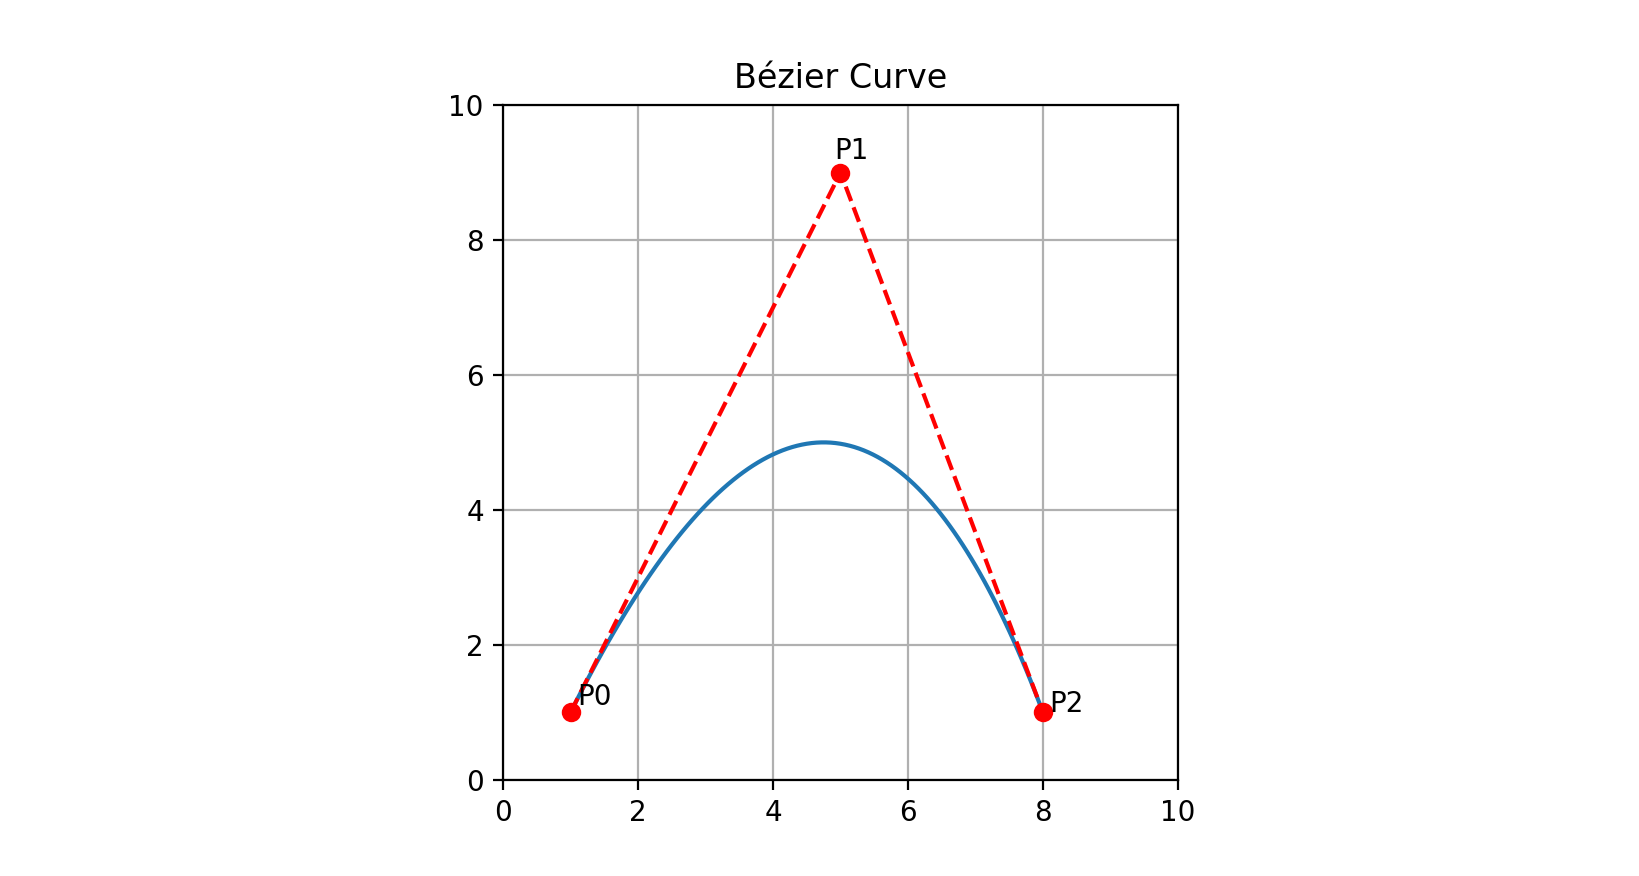
\includegraphics[width=15cm]{Figure_4}
\centering
\caption{B\'ezier curve with 3 control points, resulting from a 2nd order Bernstein polynomial.}
\end{figure}
One byproduct of how the curve is formed is that the curve always lies completely within the area bounded by the control points. The curve in Figure 7 lies completely within the triangle formed by $P_0$, $P_1$, and $P_2$.

2nd order Bernstein polynomial B\'ezier curves are referred to as quadratic Bezier curves. Another common form is the cubic B\'ezier curve, which uses a 3rd order Bernstein polynomial.
$$B(t)=(1-t)^3 P_0+3t (1-t)^2 P_1+3t^2 (1-t) P_2+t^3 P_3$$
As can be expected, a 3rd order polynomial has 4 terms and 4 control points.

\begin{figure}[H]
\centering
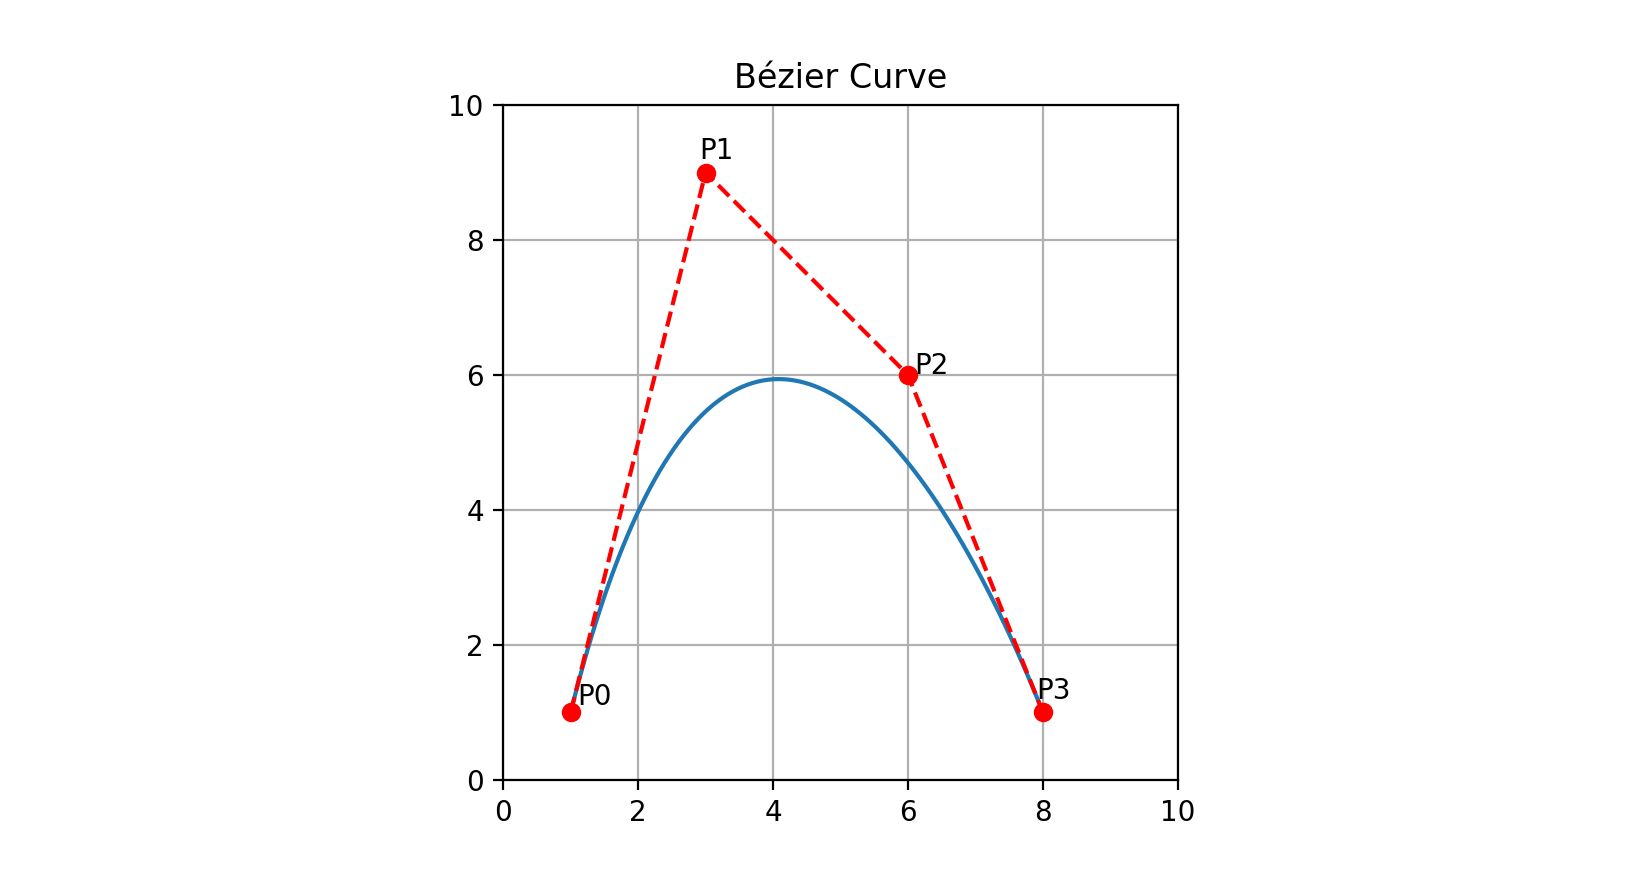
\includegraphics[width=15cm]{Figure_5}
\caption{Cubic B\'ezier curve with 4 control points, generated with a 3rd order Bernstein polynomial.}
\end{figure}

\section{Applications}

\subsection{Computer-Aided Design}

Computer-Aided Design (CAD) was the original intended application for the B\'ezier curve, so it comes by no surprise that the method is used in its graphic rendering engine. SolidWorks uses parametric geometry in its 2D sketch mode, a similar process to the B\'ezier curve. 

%talk about NURBS and their relation with Bezier and Casteljau

NURBS are the standard method for representing 3D objects and surfaces in CAD applications, including SolidWorks, Autodesk Fusion, and Autodesk Inventor. 
%more

\subsection{Fonts}

Until laser printers had a high enough dot density to produce legible text, digital fonts were essentially unnecessary and nonexistent. As printer technology developed, a digital typeface became a more and more likely end. B\'ezier curves ultimately answered the question of how to produce a digital text character with its easy to use and efficient to encode curves.

\begin{figure}[H]
\centering
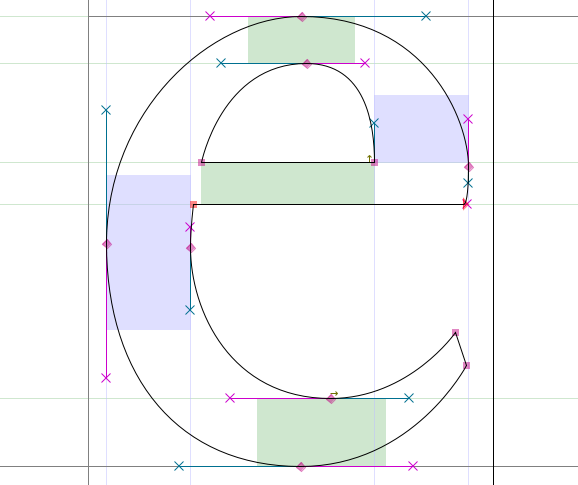
\includegraphics[width=10cm]{char}
\caption{Letter 'e' with visible B\'ezier control points}
\end{figure}

B\'ezier curves are suited well for fonts not only because computers can handle them well, but their adaptability and ease of adjustment lends toward the process of optical balancing. The design process of a font, even individual characters, requires very close attention to optical balance to make characters look and feel the way they are meant to be. Optimizing fonts is a topic for another discussion, so for now B\'ezier curves offer the flexibility needed to create quality fonts while also being efficient for computers to render. 

Computational efficiency is incredibly important for font rendering simply because text is rendered so frequently. As can be seen in the python code in Figure 9, rendering a curve is a very simple task that only requires a few numerical arguments. As the primary method of displaying information in language form on a screen, text is rendered all the time. The efficiency of the B\'ezier curve allows text to not be a heavy burden on the CPU to produce. 

The prevalence of B\'ezier curves in fonts has to do with the main digital font formats which are industry standards: TrueType and PostScript. PostScript was designed by Adobe in the early ‘80s as their core technology. It is a programming language dedicated toward document rendering. Fonts, as well as vector graphics, were drawn as a series of lines and cubic B\'ezier curves. These documents could be scaled to any resolution, and therefore were compatible with virtually any laser printer. 

Apple developed the TrueType outline font format to replace bitmap fonts in its Macintosh computers. TrueType was released with Macintosh System 7. It uses lines and quadratic B\'ezier curves. While quadratic curves aren’t as flexible as cubic with one less control point, they are computationally lighter for the same reason.

TrueType managed to become the dominant font standard after Apple licensed it to Microsoft. TrueType was added to the Windows operating system in 1991, and Microsoft published many TrueType fonts. Later on Microsoft created the OpenType format, which borrowed much of the underlying structure from TrueType, but included features for more control over typefaces. 

Both TrueType and PostScript replaced bitmap fonts entirely. Bitmap fonts were much harder to scale and less elegant than the curve-based successors. A bitmap font had to be recreated individually for each resolution, which was useful for making legibility adjustments at different sizes but was much more labor intensive to scale up or down for different sizes. Vector fonts could be automatically scaled, which is part of why they became the industry standard in digital typefaces. Now, on both Windows and macOS, TrueType, OpenType, and PostScript fonts are supported.


\subsection{Vectors}

PostScript’s use of cubic B\'ezier curves also made its way to the dominant vector graphic design software Adobe Illustrator. Illustrator relies heavily on cubic B\'ezier curves to draw most every shape. The system is based entirely around the control points of the curves. The endpoints of curves are referred to as control points, while the two points that lie off the curve are called handles. The control point-based control scheme has been adopted as the default method of interaction in vector drawing software, and can be found in Illustrator and other popular vector programs such as CorelDRAW.

\begin{figure}[H]
\centering
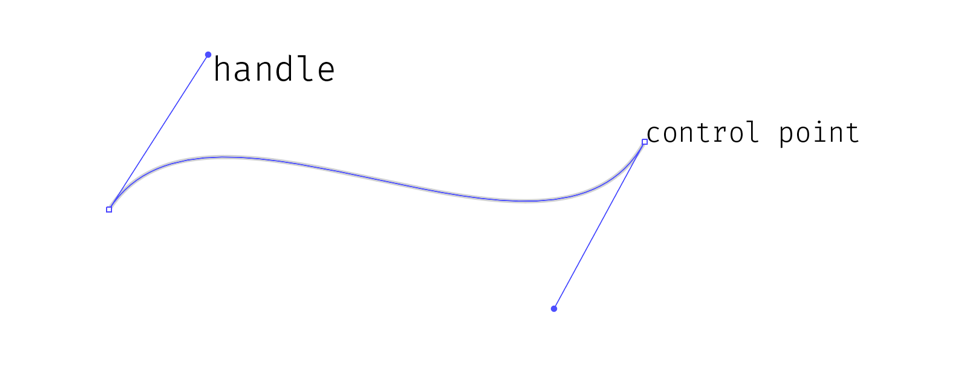
\includegraphics[width=\textwidth]{illustrator-ex}
\caption{Example curve with control points visible, drawn the pen tool in Adobe Illustrator.}
\end{figure}

The Scalable Vector Graphics file format is the common vector file format which can be read by mainstream vector software packages. It is written in XML.

\newpage
\bibliography{tynan-ee}
\bibliographystyle{apa}
\appendix
\listoffigures
\listoftables
\lstinputlisting[language=python]{../py/decasteljau.py}
\end{document}




